\addcontentsline{toc}{chapter}{Introducción}
\chapter*{Introducción}
        %\thispagestyle{empty}

    \lettrine[lines=9] {\initfamily  \selectfont E}{n} los años 1670, Gottfried Wilhelm Leibniz (1646 - 1716) escribió a Christiaan Huygens (1629 - 1695): \textit{``Necesitamos un análisis propiamente geométrico o lineal, que exprese directamente la situación (el situs), como el álgebra expresa la magnitud''.} Leibniz no estaba conforme con el enfoque geométrico de Euclides ni con el de la recién creada \textit{Geometría Analítica} de René Descartes (1596 - 1650). Su sueño era crear una especie de lenguaje universal en el que todos los teoremas pudieran ser demostrados mediante manipulaciones de algunos símbolos. Su \textit{Análisis Situs} pretendía seguir esta dirección, aunque no cosechó muchos frutos en su época. No obstante, esta idea de la \textit{Geometría de la Posición} estaría en constante búsqueda por parte de los matemáticos que sucedieron a Leibniz.
    
            \begin{wrapfigure}{r}{0.4\textwidth}
            \vspace{-0.4cm}
            \centering
            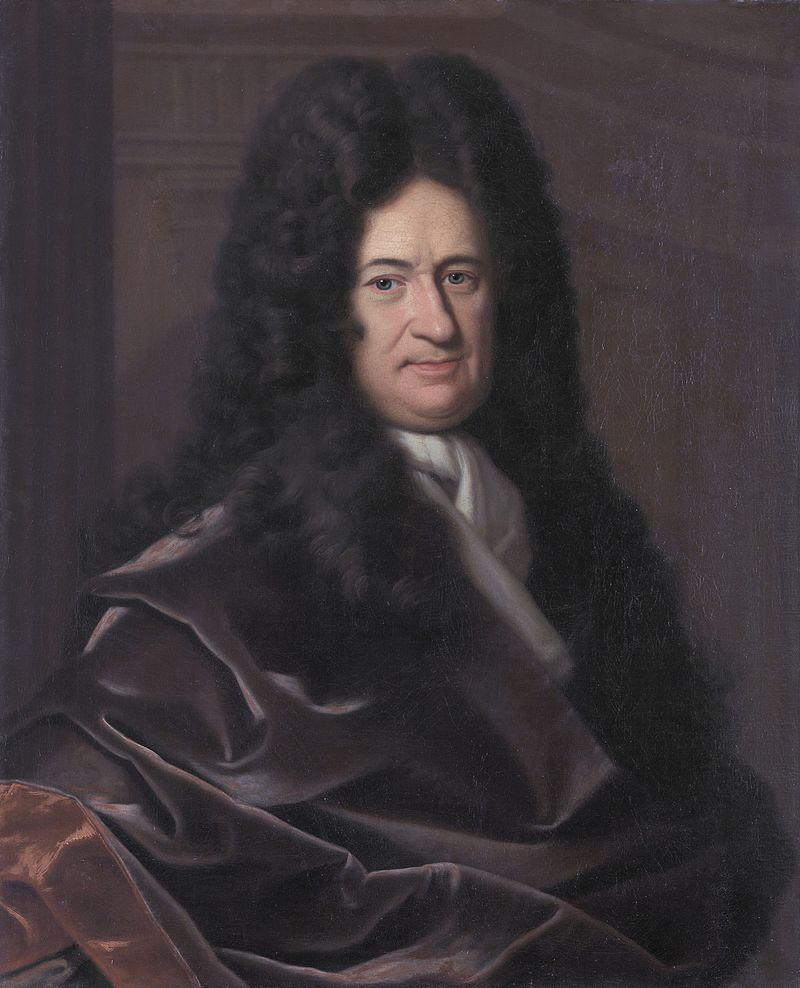
\includegraphics[scale=0.5]{img/imgintro/Gottfried_Wilhelm_Leibniz,_Bernhard_Christoph_Francke.jpg}
            \caption{Gottfried Leibniz}
            \label{fig:euler} 
            %\vspace{-0.8cm}
        \end{wrapfigure}


Se sabe que la \textit{Teoría de Gráficas} tuvo su origen en 1736 de la mano de Leonhard Euler (1707 - 1783) al resolver el famoso problema de los Puentes Königsberg (hoy Kaliningrado, Rusia). De hecho, Euler consideraba que sus nuevos métodos eran parte del ansiado Análisis Situs de Leibniz, dando inicio a lo que posteriormente se conocería como \textit{Topología}.

Respecto al \textit{Álgebra Lineal}, sus orígenes pueden rastrearse hasta las culturas babilónica y egipcia. En el mundo oriental, los matemáticos chinos lograron desarrollar métodos de resolución de sistemas de ecuaciones. 

Hallamos en Leibniz y en el matemático japonés Seki Kowa (1642 - 1708) las primeras menciones de los \textit{determinantes}. Aunque no sería hasta 1850 cuando James Joseph Sylvester (1814 - 1897) acuña por primera vez el término \textit{matriz} para designar los arreglos rectangulares de números asociados a los sistemas de ecuaciones. En esta época, Arthur Cayley (1821 - 1895) desarrolla el álgebra de matrices definiendo sus operaciones básicas así como la inversa de una matriz y su construcción. El francés Camile Jordan (1838 - 1922) también hace importantes contribuciones al respecto.

\begin{wrapfigure}{l}{0.35\textwidth}
    \vspace{-0.4cm}
    \centering
    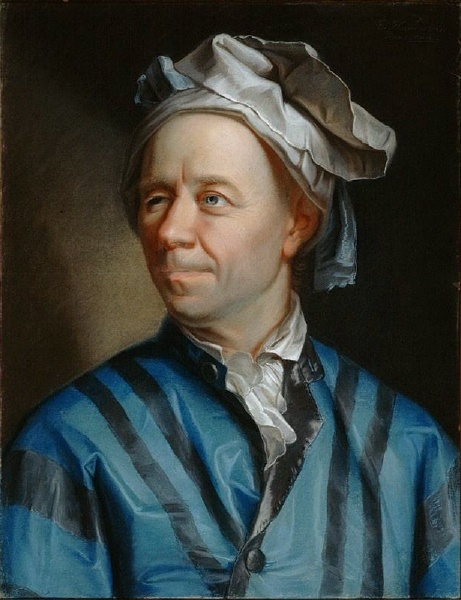
\includegraphics[scale=0.4]{img/imgintro/euler.jpg}
    \caption{Leonhard Euler}
    \label{fig:euler}   
\vspace{-0.3cm}
\end{wrapfigure}


Es curioso que tanto Sylvester, Jordan y Cayley estudiaron los \textit{árboles} de las gráficas, siendo este último el más prolífico. Debe mencionarse aquí que fue el propio Sylvester el primero en usar el término \textit{gráfica} para designar a los \textit{sistemas de puntos y líneas} (así eran llamadas las gráficas en esos tiempos).


Quizás no es tan conocido que la Teoría de Gráficas terminó por consolidarse con las contribuciones del físico alemán Gustav Robert  Kirchhoff (1824 - 1887), nacido en Königsberg. Kirchhoff estableció dos leyes fundamentales en el análisis de las \textit{redes eléctricas} que dan lugar a ciertos sistemas de ecuaciones. Para resolverlos, el físico hizo uso de la gráfica asociada a la red eléctrica y, con ayuda de los árboles generadores, construyó sistemas de ecuaciones linealmente independientes más fáciles de solucionar. Este fue de los primeros momentos en que el Álgebra Lineal y la Teoría de Gráficas se relacionaron.



Años después, Henri Poincaré retomaría estas ideas sistematizándolas en su fundamental artículo (junto con cinco suplementos) titulado \textit{Analysis Situs} y dando nacimiento a la \textit{Topología Algebraica}. Encontramos en este artículo la primera mención de la \textit{matriz de incidencia} de una gráfica.

\begin{wrapfigure}{r}{0.35\textwidth}
%\vspace{-0.5cm}
    \centering
    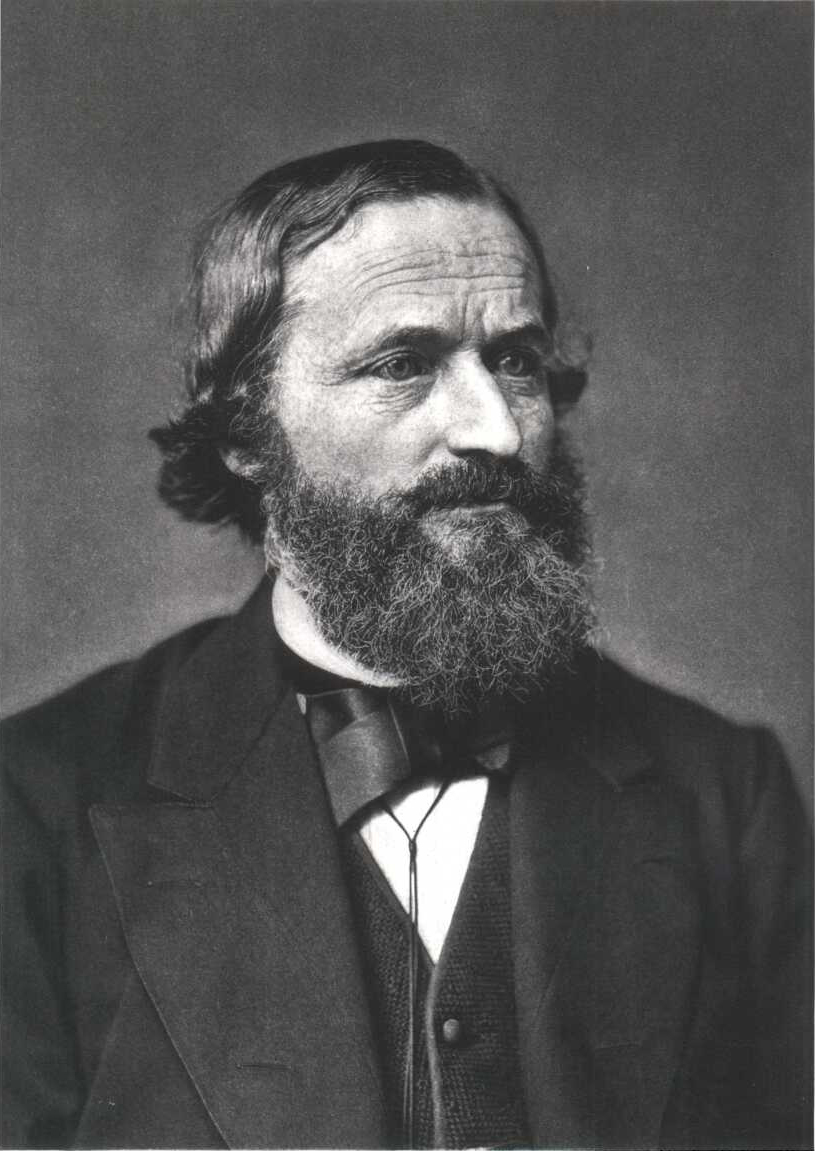
\includegraphics[scale=0.23]{img/imgintro/kirchoff.jpg}
    \caption{Gustav Kirchhoff}
    \label{fig:veblen}
 %   \vspace{-0.45cm}
\end{wrapfigure}

A su vez, el matemático estadounidense Oswald Veblen (1880 - 1960) retomó el trabajo de Poincaré y publicó en 1922 un libro llamado también \textit{Analysis Situs}. Fue el primer libro de texto de Topología en inglés. Entre sus muy diversas contribuciones, se encuentran por primera vez sistematizados los conceptos de Teoría de Gráficas junto con el Álgebra Lineal. Aquí se hace mención, por ejemplo, del \textit{rango} y la \textit{nulidad} de una gráfica como las dimensiones, respectivamente, del espacio de renglones y el espacio nulo de la matriz de incidencia de la gráfica. Veblen también aportó al estudio de las gráficas planas, de los ciclos y en el \textit{Problema de los Cuatro Colores}.


En los años 1930, Hassler Whitney (1907 - 1989) se interesó también en el Problema de Los Cuatro Colores y en hallar una caracterización combinatoria de las gráficas planas. Para ésto, Whitney utilizó conceptos algebraicos como los mencionados en el libro de Veblen. Logró darse cuenta de varias similitudes entre los espacios vectoriales y las subgráficas de una gráfica dada y generalizó estas relaciones en unas nuevas estructuras que llamó \textit{matroides}.

Después de la Segunda Guerra Mundial, se produjo un desarrollo en la Programación Lineal gracias a George B. Dantzig y su \textit{Método Simplex}. Este acontecimiento provocó el surgimiento de la Optimización Combinatoria (que ya venía gestándose paralelamente a la Teoría de Gráficas) como disciplina en los años 50, donde los matroides encontraron sus aplicaciones más importantes.

La historia de la Teoría de Gráficas está documentada (con todo detalle) en el libro de Biggs, Lloyd y Wilson \cite{Biggs}.  


\begin{figure}
\begin{subfigure}{0.5\textwidth}
    \centering
    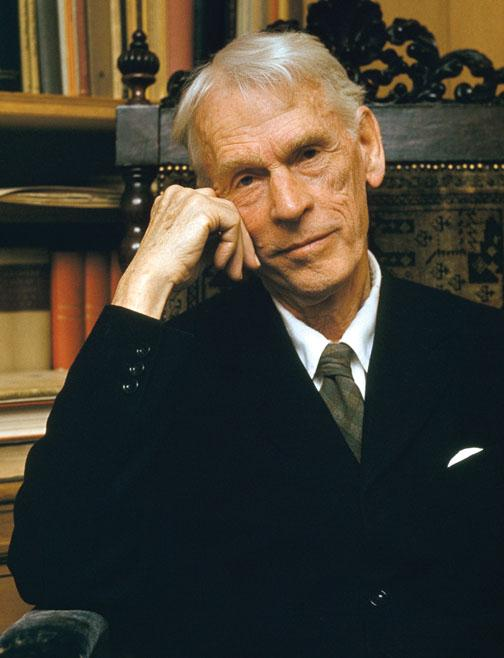
\includegraphics[scale=0.55]{img/imgintro/veblen.jpg}
    \caption{Oswald Veblen}
    \label{fig:my_label}
\end{subfigure}
\begin{subfigure}{0.5\textwidth}
    \centering
    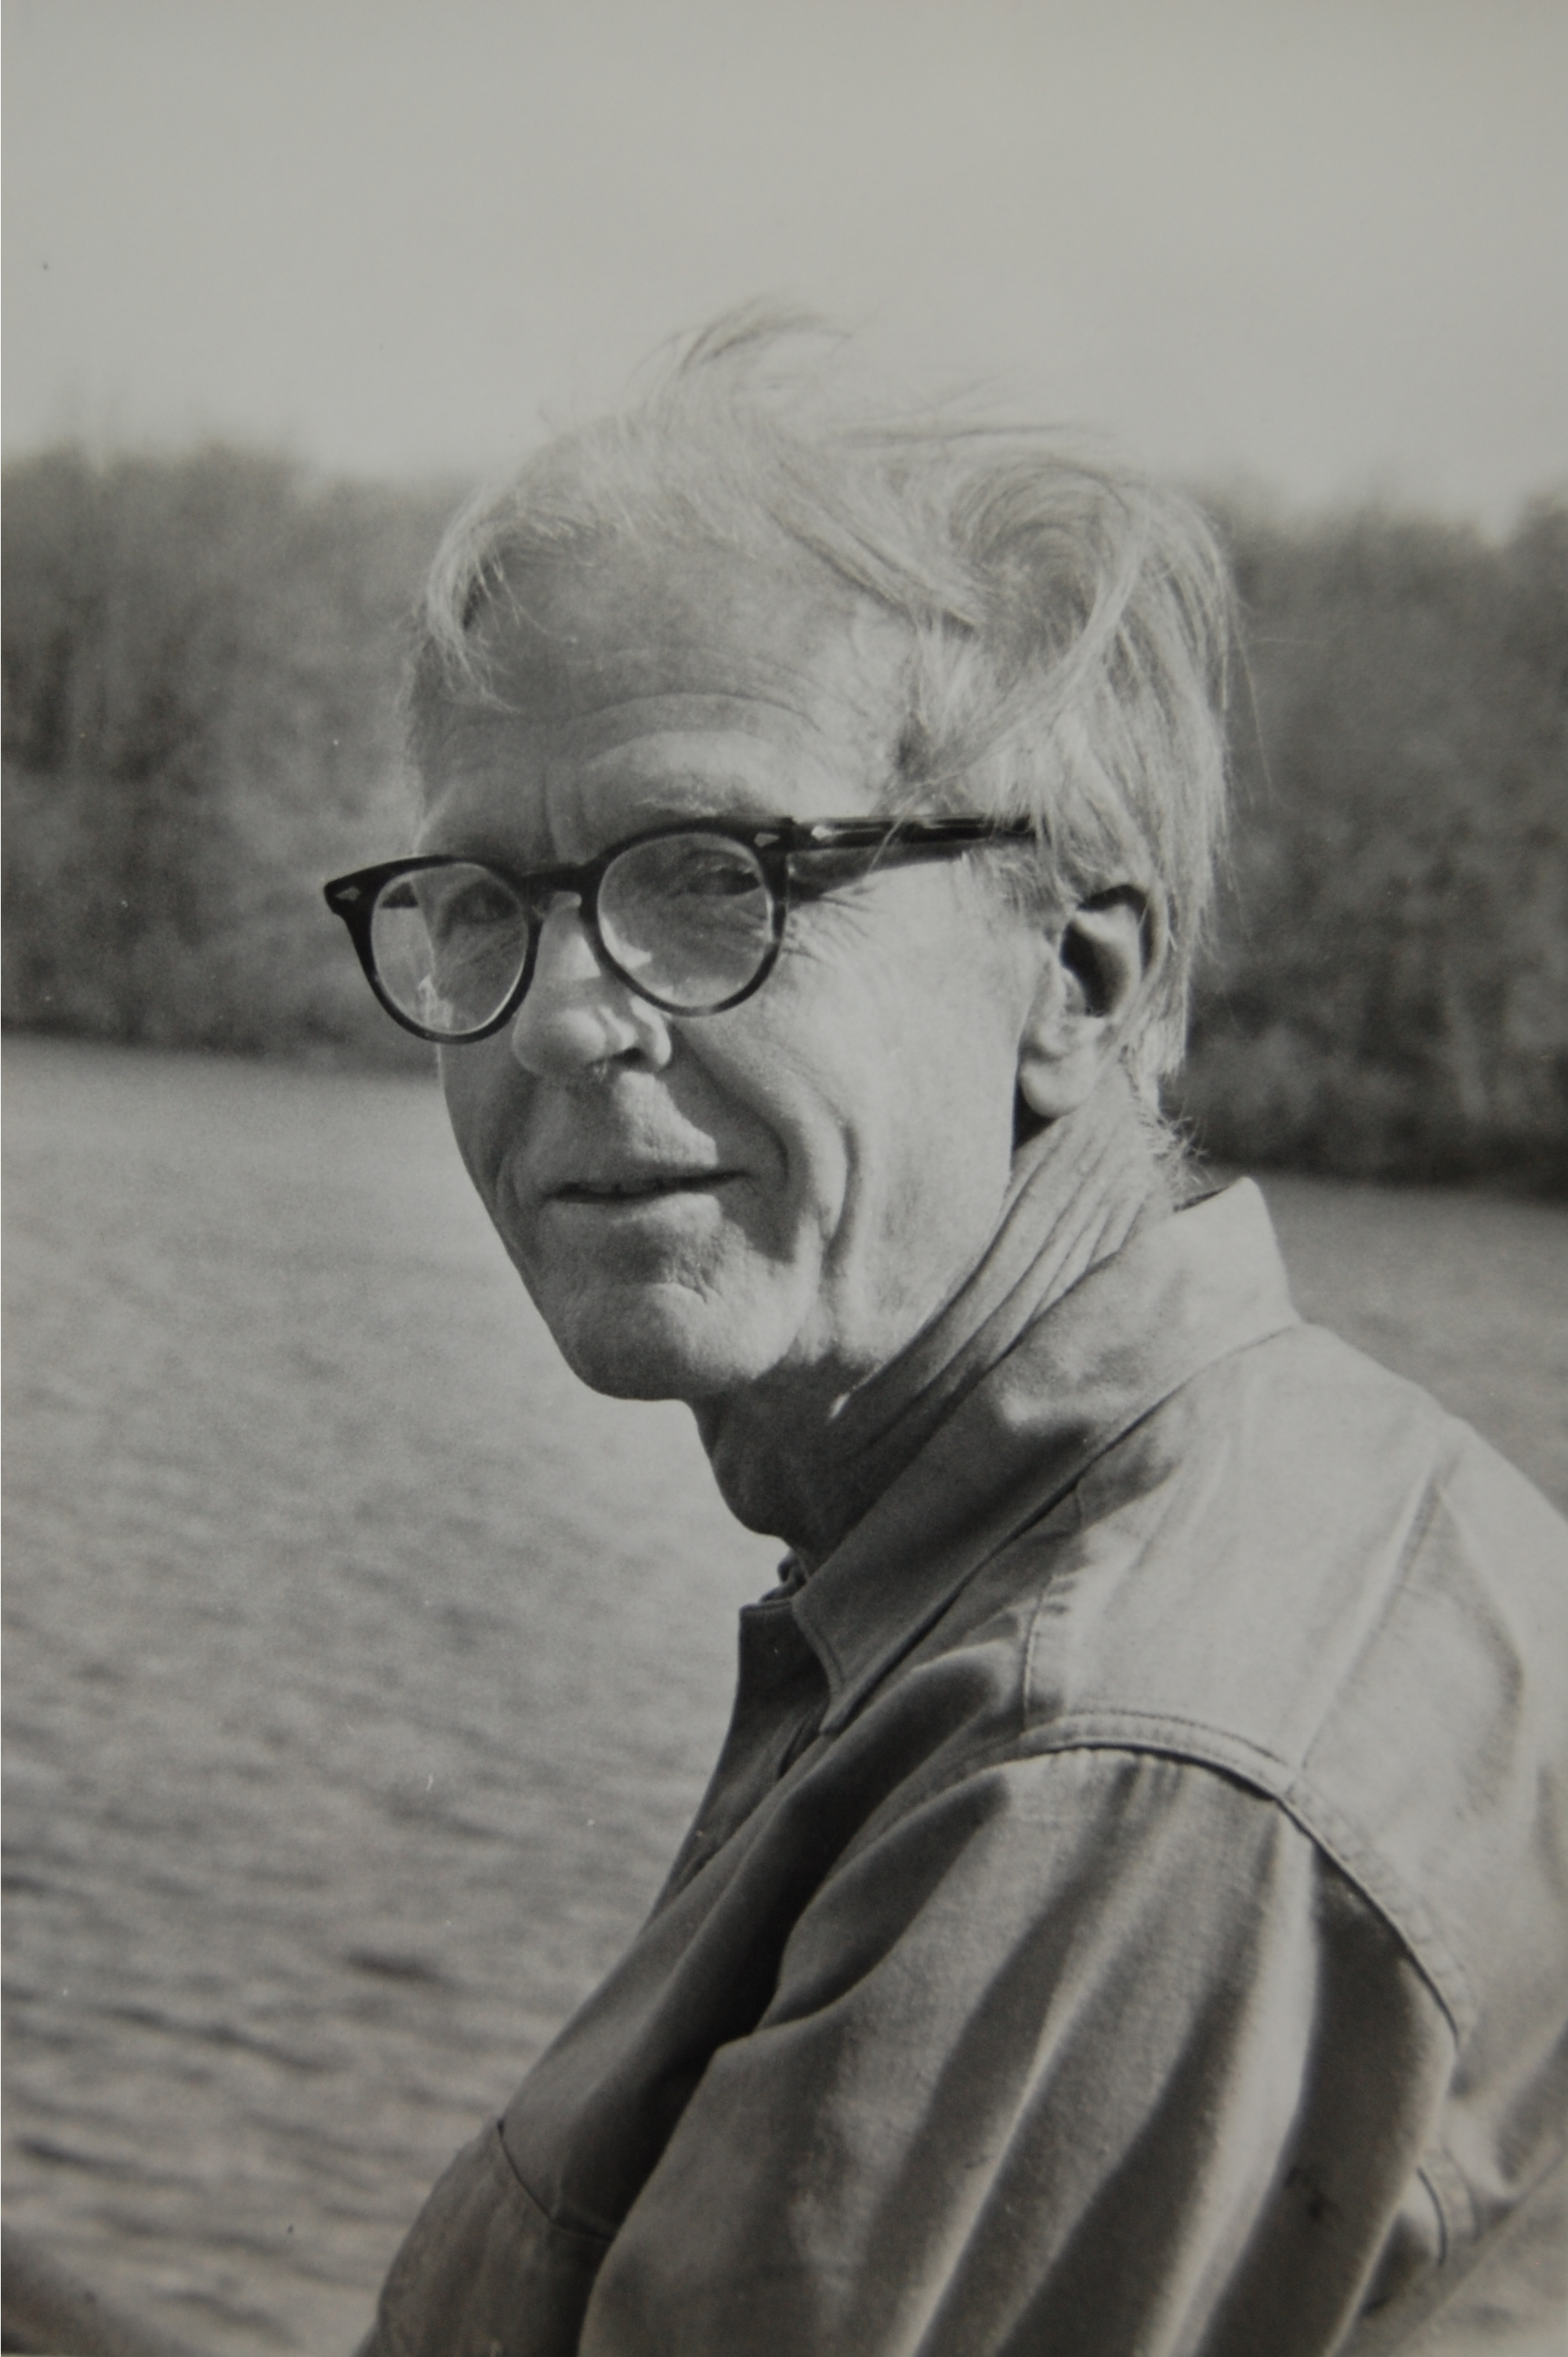
\includegraphics[scale=0.4]{img/imgintro/whitney.jpg}
    \caption{Hassler Whitney}
    %\label{fig:my_label}
\end{subfigure}
\end{figure}


